\documentclass[10pt]{article}
\setlength{\textwidth}{6.85in}
\setlength{\oddsidemargin}{-0.35in}
\setlength{\topmargin}{-1.0in}
\setlength{\textheight}{9.7in}
\setlength{\footskip}{1.0in}
\usepackage{amssymb}
\usepackage{amsthm}
\usepackage{amsmath}
\usepackage{bm}
\usepackage{latexsym}
\usepackage{mathtools}
\usepackage[dvipdfmx]{graphicx}
\usepackage[dvipdfmx]{color}
\usepackage[dvipdfmx, colorlinks=true, allcolors=blue]{hyperref}
\usepackage{listings}
\usepackage{physics}
\usepackage{url}
\usepackage{wrapfig}

\renewcommand{\refname}{参考文献}
\renewcommand{\baselinestretch}{1.0}

\begin{document}

\begin{center}
    \begin{LARGE}
        書類選考課題解答(修士課程用)
    \end{LARGE}
    \vspace{0.5cm}
    受験者氏名: -- --\\
\end{center}

\noindent
{\bf 課題1.}\\

\noindent
{\bf 研究テーマ:}再帰的構造を有する密行列を利用した高速な行列のsketching\\

\noindent
{\bf (本文)}\\

私が修士課程において行いたい研究テーマは様々あるが、その内の一つが\textbf{行列のsketching}である。

\noindent
{\bf \textcolor{magenta}{このテーマの背景}}

初めに、このテーマの背景であるsketchingとは、一体どのようなものなのかについて述べる。これは、近年発展してきたデータ圧縮技法の一つであり、非常に大規模な行列$A \in \mathbb{R}^{n \times d} \: (n \gg d)$に対して、一定の確率、および、一定の割合のもとでその性質(ベクトル積との$L^2$ノルムなど)を保持するような、より小さい行列$B$を求めることを指す。そのような操作をすることで、大規模なデータを、現実的に計算可能なサイズにまで落とした上で、より高速に最適化などを行うことが可能となる\cite{falconeMatrixSketchingSupervised2019}。

代表的な手法の一つに、\textbf{sparse matrix}を用いたsketchingが挙げられる\cite{woodruffSketchingToolNumerical2014}。
sparse matrixとは、Fig\ref{img:JLT_S}に示したような、各列に$\pm1$の内のどちらかが、ランダムに丁度一つ存在するような疎行列である。そして、このようなdata obliviousな行列であっても、一定のパラメータの下で、Johnson-Lindenstrauss Transform(JLT)になるということが知られている。つまり、
\begin{align*}
    S \; \mathrm{is} \; JLT(\epsilon, \delta, f) \Leftrightarrow
    |\langle Sv,Sv' \rangle - \langle v,v' \rangle| \leq \epsilon ||v||_2 ||v'||_2 \quad (\mathrm{with\;probability\;}1-\delta) \quad (v,v'\in f\mathrm{-element} \; \mathrm{subset} \; V \subset \mathbb{R}^n)
\end{align*}
となる\cite{woodruffSketchingToolNumerical2014}。このような性質を持つ行列$S$(Fig\ref{img:JLT_S})などを用いて、行列$A$(Fig\ref{img:JLT_A})の性質を、その部分空間である行列$B=SA$(Fig\ref{img:JLT_SA})に埋め込む。これが、sparse matrixを用いたsketchingの基本的な考え方である。

\begin{figure}[htbp]
    \begin{minipage}{0.6\hsize}
        \begin{center}
            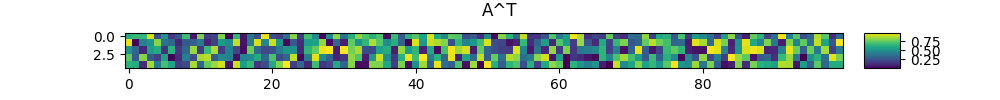
\includegraphics[width=\hsize]{sparseMatrix_At.png}
        \end{center}
        \caption{sketchingの対象となる行列$A$の転置}
        \label{img:JLT_A}
    \end{minipage}
    \begin{minipage}{0.4\hsize}
        \begin{center}
            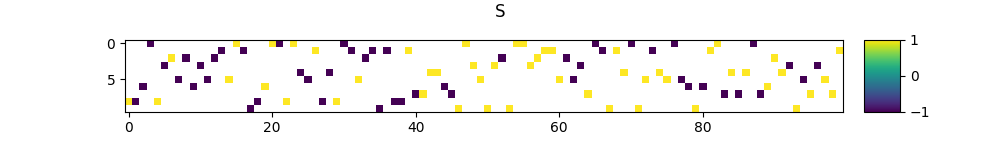
\includegraphics[width=\hsize]{sparseMatrix_S.png}
        \end{center}
        \caption{sparse matrix $S$}
        \label{img:JLT_S}
    \end{minipage}
\end{figure}

\begin{wrapfigure}{r}[0pt]{0.2\textwidth}
    \vspace{-1.5\baselineskip}
    \begin{center}
        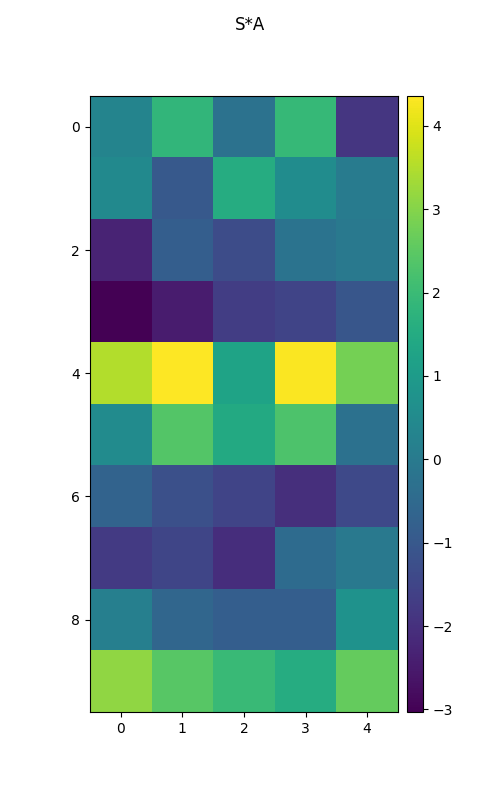
\includegraphics[width=0.2\textwidth]{sparseMatrix_SA.png}
        \caption{embeddingされた行列$SA$}
        \label{img:JLT_SA}
    \end{center}
    \vspace{-1.5\baselineskip}
\end{wrapfigure}

\noindent
{\bf \textcolor{magenta}{近年の進展状況}}

先程はsparse matrixを掛け合わせる手法を取り上げたが、matrix sketchingには他にも様々な手法がある。一つは、element-wiseに行列の要素を取って来て、全体の形はそのままに疎行列にする方法がある\cite{kunduNoteRandomizedElementwise2014}。また、後述のように、幾つかの列を組み合わせながら作成していく方法などもある。そして、それぞれの方面で、盛んな研究が行われており、相互に影響を与えながら進展しているといった印象を受けている。

また、特に近年で言えば、機械学習分野など、大規模なデータを扱う分野の盛り上がりに呼応して、pass-efficientやstreamingなどと言った語が登場するようになってきている。則ち、データを何回か、あるいは、1回だけしか読み込まないということである。全体をそのままは保持できないような非常に大規模なデータを扱う際、情報の収集と同時にsketchingをしてしまえば、メモリを節約し、かつ、全体の性質を保持したまま、データを扱うことが可能となる\cite{libertySimpleDeterministicMatrix2013}。なので、このような状況下でのsketchingも盛んになり始めているようである。

大規模データの効率的な取り扱いの重要性は日ごとに増しているが、そのような場面においてこそ、行列のsketchingは真価を発揮すると考えており、今後のさらなる発展が期待される分野であると言えるだろう。そして、それ故に、この分野の研究を視野に入れている。

\noindent
{\bf \textcolor{magenta}{自分なりの着想・構想}}

最後に、私個人の観点からの展望を述べる。

一つ大きく注目している点が、\textbf{Walsh行列}(Fig\ref{img:Walsh})を利用したsketchingである。
詳細は省くが、このWalsh行列$H_n$に対し、対角成分にランダムに$\pm1$が入る対角行列$D$との積$H_nD$を考えると、各列は独立な$\pm1$からなるvectorであり、かつ、行列全体としてもfull rankなので、Chernoffの不等式(適切な設定の下で、$P(X \geq a ) \leq \frac{E(e^{tX})}{e^{ta}}$)と似た議論により、$\max_{||\bm{x}||_2=1}||H_nD\bm{x}||_{\infty}$がとある定数オーダーで抑えられることが分かる。直感的には、$H_n$が密行列であることから、$H_nD\bm{x}$の要素は、$\bm{x}$の各成分が互いに打ち消し合うように合算された値となり、比較的小さい値に抑えられていると解釈出来る。そして、この性質と、Walsh行列の高速な演算を可能にさせるFFT likeなアルゴリズムである高速アダマール変換を用いたsketchingが、Subsampled Randomized Hadamard Transformという従来手法である\cite{falconeMatrixSketchingSupervised2019}\cite{woodruffSketchingToolNumerical2014}\cite{ailonFastJohnsonLindenstrauss2009}。

\begin{wrapfigure}{r}[0pt]{0.2\textwidth}
    \vspace{-1.5\baselineskip}
    \begin{center}
        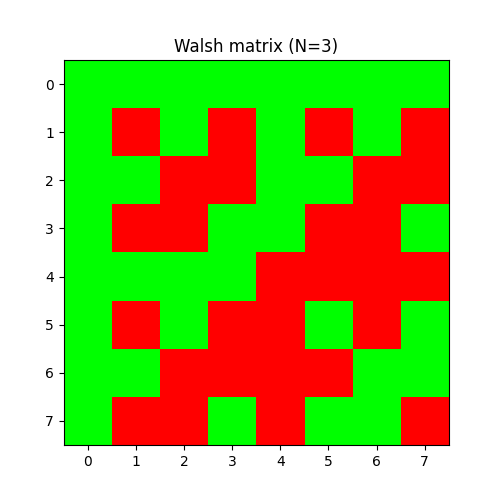
\includegraphics[width=0.2\textwidth]
        {walsh.png}
        \caption{\newline
            Walsh matrix\newline
            green:$+\frac{1}{\sqrt{2^n}}$,red:$-\frac{1}{\sqrt{2^n}}$}
        \label{img:Walsh}
    \end{center}
    \vspace{-1.5\baselineskip}
\end{wrapfigure}

しかし、Walsh行列以外にも、高速に演算可能な密行列は数多く存在している。そして、それらの行列の利用はまだあまり検討されていないのではないかとも感じた。疎行列が高速な演算を行えることは自明だが、密行列であっても、場合によっては非常に高速だというのは、なかなか非自明で興味深いことであるように思われる。なので、今後の研究の一つの方向性として、そのような、密行列を利用したsketchingの研究を行いたいと考えている。

(以下個人情報に少し関わる部分だったので削除)
\colorbox{black}{--}
\colorbox{black}{--}
\colorbox{black}{--}
\colorbox{black}{--}
\colorbox{black}{--}
\colorbox{black}{--}
\colorbox{black}{--}
\colorbox{black}{--}
\colorbox{black}{--}
\colorbox{black}{--}
\colorbox{black}{--}
\colorbox{black}{--}
\colorbox{black}{--}
\colorbox{black}{--}
\colorbox{black}{--}
\colorbox{black}{--}
\colorbox{black}{--}
\colorbox{black}{--}
\colorbox{black}{--}
\colorbox{black}{--}
\colorbox{black}{--}
\colorbox{black}{--}
\colorbox{black}{--}
\colorbox{black}{--}
\colorbox{black}{--}
\colorbox{black}{--}
\colorbox{black}{--}
\colorbox{black}{--}
\colorbox{black}{--}
\colorbox{black}{--}
\colorbox{black}{--}
\colorbox{black}{--}
\colorbox{black}{--}
\colorbox{black}{--}
\colorbox{black}{--}
\colorbox{black}{--}
\colorbox{black}{--}
\colorbox{black}{--}
\colorbox{black}{--}
\colorbox{black}{--}
\colorbox{black}{--}
\colorbox{black}{--}
\colorbox{black}{--}
\colorbox{black}{--}
\colorbox{black}{--}
\colorbox{black}{--}
\colorbox{black}{--}
\colorbox{black}{--}
\colorbox{black}{--}
\colorbox{black}{--}
\colorbox{black}{--}
\colorbox{black}{--}
\colorbox{black}{--}
\colorbox{black}{--}
\colorbox{black}{--}
\colorbox{black}{--}
\colorbox{black}{--}
\colorbox{black}{--}
\colorbox{black}{--}
\colorbox{black}{--}
\colorbox{black}{--}
\colorbox{black}{--}
\colorbox{black}{--}
\colorbox{black}{--}
\colorbox{black}{--}
\colorbox{black}{--}
\colorbox{black}{--}
\colorbox{black}{--}
\colorbox{black}{--}
\colorbox{black}{--}
\colorbox{black}{--}
\colorbox{black}{--}
\colorbox{black}{--}
\colorbox{black}{--}
\colorbox{black}{--}
\colorbox{black}{--}
\colorbox{black}{--}
\colorbox{black}{--}
\colorbox{black}{--}
\colorbox{black}{--}
\colorbox{black}{--}
\colorbox{black}{--}
\colorbox{black}{--}
\colorbox{black}{--}
\colorbox{black}{--}
\colorbox{black}{--}
\colorbox{black}{--}
\colorbox{black}{--}
\colorbox{black}{--}
\colorbox{black}{--}
\colorbox{black}{--}
\colorbox{black}{--}
\colorbox{black}{--}
\colorbox{black}{--}
\colorbox{black}{--}
\colorbox{black}{--}
\colorbox{black}{--}
\colorbox{black}{--}
\colorbox{black}{--}
\colorbox{black}{--}
\colorbox{black}{--}
\colorbox{black}{--}
\colorbox{black}{--}
\colorbox{black}{--}
\colorbox{black}{--}
\colorbox{black}{--}
\colorbox{black}{--}
\colorbox{black}{--}
\colorbox{black}{--}
\colorbox{black}{--}
\colorbox{black}{--}
\colorbox{black}{--}
\colorbox{black}{--}
\colorbox{black}{--}
\colorbox{black}{--}
\colorbox{black}{--}
\colorbox{black}{--}
\colorbox{black}{--}
\colorbox{black}{--}
\colorbox{black}{--}
\colorbox{black}{--}
\colorbox{black}{--}
\colorbox{black}{--}
\colorbox{black}{--}
\colorbox{black}{--}
\colorbox{black}{--}
\colorbox{black}{--}
\colorbox{black}{--}
\colorbox{black}{--}
\colorbox{black}{--}
\colorbox{black}{--}
\colorbox{black}{--}
\colorbox{black}{--}
\colorbox{black}{--}
\colorbox{black}{--}
\colorbox{black}{--}
\colorbox{black}{--}
\colorbox{black}{--}
\colorbox{black}{--}
\colorbox{black}{--}
\colorbox{black}{--}
\colorbox{black}{--}
\colorbox{black}{--}
\colorbox{black}{--}
\colorbox{black}{--}
\colorbox{black}{--}
\colorbox{black}{--}
\colorbox{black}{--}
\colorbox{black}{--}
\colorbox{black}{--}
\colorbox{black}{--}
\colorbox{black}{--}
\colorbox{black}{--}
\colorbox{black}{--}
\colorbox{black}{--}
\colorbox{black}{--}
\colorbox{black}{--}
\colorbox{black}{--}
\colorbox{black}{--}
\colorbox{black}{--}
\colorbox{black}{--}
\colorbox{black}{--}
\colorbox{black}{--}
\colorbox{black}{--}
\colorbox{black}{--}
\colorbox{black}{--}
\colorbox{black}{--}
\colorbox{black}{--}
\colorbox{black}{--}
\colorbox{black}{--}
\colorbox{black}{--}
\colorbox{black}{--}
\colorbox{black}{--}
\colorbox{black}{--}
\colorbox{black}{--}
\colorbox{black}{--}
\colorbox{black}{--}
\colorbox{black}{--}
\colorbox{black}{--}
\colorbox{black}{--}
\colorbox{black}{--}
\colorbox{black}{--}
\colorbox{black}{--}
\colorbox{black}{--}
\colorbox{black}{--}
\colorbox{black}{--}
\colorbox{black}{--}
\colorbox{black}{--}
\colorbox{black}{--}
\colorbox{black}{--}
\colorbox{black}{--}
\colorbox{black}{--}
\colorbox{black}{--}
\colorbox{black}{--}
\colorbox{black}{--}
\colorbox{black}{--}
\colorbox{black}{--}
\colorbox{black}{--}
\colorbox{black}{--}
\colorbox{black}{--}
\colorbox{black}{--}
\colorbox{black}{--}
\colorbox{black}{--}
\colorbox{black}{--}
\colorbox{black}{--}
\colorbox{black}{--}
\colorbox{black}{--}
\colorbox{black}{--}
\colorbox{black}{--}
\colorbox{black}{--}
\colorbox{black}{--}
\colorbox{black}{--}
\colorbox{black}{--}
\colorbox{black}{--}
\colorbox{black}{--}
\colorbox{black}{--}
\colorbox{black}{--}
\colorbox{black}{--}
\colorbox{black}{--}
\colorbox{black}{--}
\colorbox{black}{--}
\colorbox{black}{--}
\colorbox{black}{--}
\colorbox{black}{--}
\colorbox{black}{--}
\colorbox{black}{--}
\colorbox{black}{--}
\colorbox{black}{--}
\colorbox{black}{--}
\colorbox{black}{--}
\colorbox{black}{--}
\colorbox{black}{--}
\colorbox{black}{--}
\colorbox{black}{--}
\colorbox{black}{--}
\colorbox{black}{--}
\colorbox{black}{--}
\colorbox{black}{--}
\colorbox{black}{--}
\colorbox{black}{--}
\colorbox{black}{--}
\colorbox{black}{--}
\colorbox{black}{--}
\colorbox{black}{--}
\colorbox{black}{--}
\colorbox{black}{--}
\colorbox{black}{--}
\colorbox{black}{--}
\colorbox{black}{--}
\colorbox{black}{--}
\colorbox{black}{--}
\colorbox{black}{--}
\colorbox{black}{--}
\colorbox{black}{--}
\colorbox{black}{--}
\colorbox{black}{--}
\colorbox{black}{--}
\colorbox{black}{--}
\colorbox{black}{--}
\colorbox{black}{--}
\colorbox{black}{--}
\colorbox{black}{--}
\colorbox{black}{--}
\colorbox{black}{--}
\colorbox{black}{--}
\colorbox{black}{--}
\colorbox{black}{--}
\colorbox{black}{--}
\colorbox{black}{--}
\colorbox{black}{--}
\colorbox{black}{--}
\colorbox{black}{--}
\colorbox{black}{--}
\colorbox{black}{--}
\colorbox{black}{--}
\colorbox{black}{--}
\colorbox{black}{--}
\colorbox{black}{--}
\colorbox{black}{--}
\colorbox{black}{--}
\colorbox{black}{--}
\colorbox{black}{--}
\colorbox{black}{--}
\colorbox{black}{--}
\colorbox{black}{--}
\colorbox{black}{--}
\colorbox{black}{--}
\colorbox{black}{--}
\colorbox{black}{--}
\colorbox{black}{--}
\colorbox{black}{--}
\colorbox{black}{--}
\colorbox{black}{--}
\colorbox{black}{--}
\colorbox{black}{--}
\colorbox{black}{--}
\colorbox{black}{--}
\colorbox{black}{--}
\colorbox{black}{--}
\colorbox{black}{--}
\colorbox{black}{--}
\colorbox{black}{--}
\colorbox{black}{--}
\colorbox{black}{--}
\colorbox{black}{--}
\colorbox{black}{--}
\colorbox{black}{--}
\colorbox{black}{--}
\colorbox{black}{--}
\colorbox{black}{--}
\colorbox{black}{--}
\colorbox{black}{--}
\colorbox{black}{--}
\colorbox{black}{--}
\colorbox{black}{--}
\colorbox{black}{--}
\colorbox{black}{--}
\colorbox{black}{--}
\colorbox{black}{--}
\colorbox{black}{--}
\colorbox{black}{--}
\colorbox{black}{--}
\colorbox{black}{--}
\colorbox{black}{--}
\colorbox{black}{--}
\colorbox{black}{--}
\colorbox{black}{--}
\colorbox{black}{--}
\colorbox{black}{--}
\colorbox{black}{--}
\colorbox{black}{--}
\colorbox{black}{--}
\colorbox{black}{--}
\colorbox{black}{--}
\colorbox{black}{--}
\colorbox{black}{--}
\colorbox{black}{--}
\colorbox{black}{--}
\colorbox{black}{--}
\colorbox{black}{--}
\colorbox{black}{--}
\colorbox{black}{--}
\colorbox{black}{--}
\colorbox{black}{--}
\colorbox{black}{--}
\colorbox{black}{--}
\colorbox{black}{--}
\colorbox{black}{--}
\colorbox{black}{--}
\colorbox{black}{--}
\colorbox{black}{--}
\colorbox{black}{--}
\colorbox{black}{--}
\colorbox{black}{--}
\colorbox{black}{--}
\colorbox{black}{--}
\colorbox{black}{--}
\colorbox{black}{--}
\colorbox{black}{--}
\colorbox{black}{--}
\colorbox{black}{--}
\colorbox{black}{--}
\colorbox{black}{--}
\colorbox{black}{--}
\colorbox{black}{--}
\colorbox{black}{--}
\colorbox{black}{--}
\colorbox{black}{--}
\colorbox{black}{--}
\colorbox{black}{--}
\colorbox{black}{--}
\colorbox{black}{--}
\colorbox{black}{--}
\colorbox{black}{--}
\colorbox{black}{--}
\colorbox{black}{--}
\colorbox{black}{--}
\colorbox{black}{--}
\colorbox{black}{--}
\colorbox{black}{--}
\colorbox{black}{--}
\colorbox{black}{--}
\colorbox{black}{--}

\noindent
{\bf 課題2.}\\

\noindent
{\bf 重要な事項:}特異値分解\\

\noindent
{\bf (1)数理的な詳細}

特異値分解とは、行列分解の手法の一つであり、任意の実行列$A \in \mathbb{R}^{n \times m}$を$A = U \Sigma V^T$と分解することを指す。ただし、$U \in \mathbb{R}^{n \times n}$と$V \in \mathbb{R}^{m \times m}$は直交行列であり、$\Sigma$は特異値を(一般的には降順に)対角成分に並べた行列である(なお、行列は必ずしも実行列である必要はなく、体$K$の元であれば良いが、ここでは実数に限って議論を進める)。
ここで登場した特異値にはいくつか重要な性質が存在し、行列$A$の階数と非零の特異値の個数が一致すること、特異値が$A^TA$の固有値と一致すること、特異値の二乗和はフロベニウスノルム$||A||_F$の二乗に一致すること($\because ||A||_F=\sum_{i,j}|a_{ij}|^2=\tr(A^TA)$)などが挙げられる。他にも重要な性質は多数存在するが、実用と結びついた説明の方が良いと考え、本問(2)にその他多くを記した。
また、特異値分解は、一般には$\order{n^3}$の計算量を要するが、近年では実質的に$\order{n^2}$の計算量で求める手法なども提案されている\cite{YouZuoTeYiZhiFenJiearugorizumunoZuiJinnoFaZhan2014}。

\noindent
{\bf (2)数理情報学における意義}

特異値分解は、数理情報学において極めて頻出の手法であり、実際、計数工学科における授業内でも、幾度となく登場している。本節では、各分野に沿ってその意義を述べる。

\noindent
{\bf \textcolor{magenta}{線形代数-条件数}}\quad
行列の作用素ノルム$||A||_p=\sup_{\bm{x} \neq 0}\frac{||A\bm{x}||_p}{||\bm{x}||_p}$は、$p=2$の場合、$A$の最大特異値に一致することが知られている。これは、特異値分解した際の直交行列$U,V$に関して、それらをベクトルに掛けてもノルムが不変という性質から導かれる。また、行列の条件数$\kappa_p(A)=||A||_p||A^{-1}||_p$は、同様の理論から$A$の最大特異値と最小特異値の比に一致することが分かる。ここで、条件数は、$\sup_{\bm{b} \neq 0}\frac{||\bm{b}||_2}{||A^{-1}b||_2} \cdot \sup_{\bm{\Delta b} \neq 0}\frac{||A^{-1}\bm{\Delta b}||_2}{||\bm{\Delta b}||_2}$とも表せ、これは連立方程式$A(x_{\bm{b}}+x_{\bm{\Delta b}})=\bm{b}+\bm{\Delta b}$における誤差項$\bm{\Delta b}$の鋭敏性を評価している。このように、条件数は数値解析において行列の安定性を表す指標として用いられており、特異値分解と合わせて重要と言える\cite{SongWeiShuZhiJieXiDi2ZhangXianXingFangChengShiLianLiYiCiFangChengShi2021}。

\noindent
{\bf \textcolor{magenta}{画像処理-逆問題}}\quad

\begin{wrapfigure}{r}[0pt]{0.4\textwidth}
    \vspace{-1.5\baselineskip}
    \begin{center}
        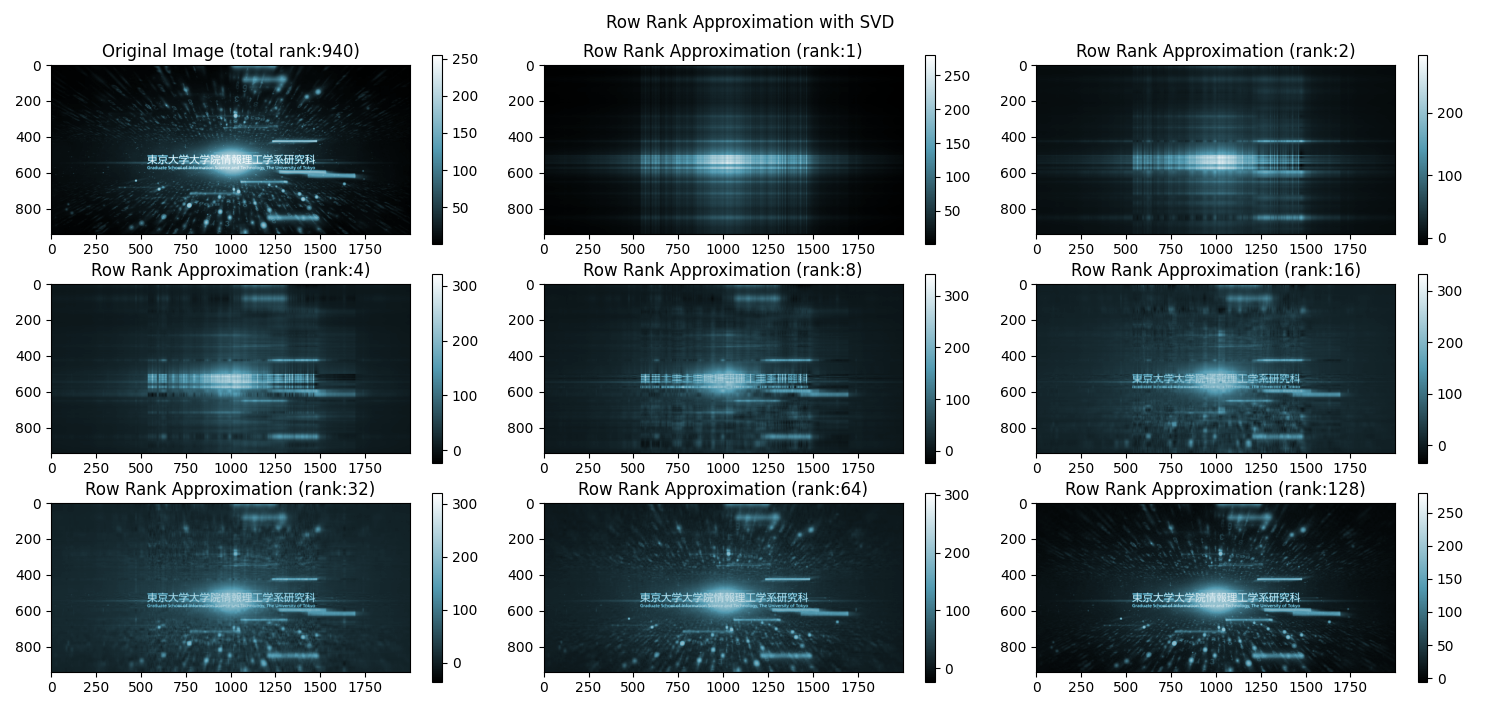
\includegraphics[width=0.4\textwidth]{RowRankImage.png}
        \caption{画像の低ランク近似}
        \label{img:RowRankImage}
    \end{center}
    \vspace{-1.5\baselineskip}
\end{wrapfigure}

特異値分解の重要な応用の一つに、Moore-Penroseの一般化逆行列が挙げられる。
この行列は、$A^+ = V \Sigma^+ U^T$と計算することが出来る。ただし、$\Sigma^+$は、長方対角行列であり、$\Sigma$の対角成分の非零要素を逆数にして転置したものとする。このような行列は、最小二乗問題において、ユークリッドノルム最小の解を与えることなどで知られ、画像のボケ除去などの不良設定問題で応用がある。
また、同じく逆問題として、数理工学特論第二など、データ同化やカルマンフィルタなどの文脈においてもこの一般化逆行列は登場することが知られている\cite{GengJieNiWenTitositeno4CiYuandetaTongHua2020}。

なお、特異値分解は低ランク近似にも用いられており、ある階数$r'(\leq r)$での、2ノルム、および、フロベニウスノルムの意味での最良近似行列は、$A$の特異値分解において、最大$r'$個の特異値を残したものであることが知られている(Eckart-Young-Mirsky Theorem)\cite{wilkinsonLowrankApproximationMultivariate}。
このことから、画像の圧縮にも使用することが可能である。Fig\ref{img:RowRankImage}に示した特異値分解による画像の低ランク近似の実験結果では、rank=16程度でも十分復元出来ており、rank=128では元画像とほぼ同等になる。元画像は\href{https://www.i.u-tokyo.ac.jp/}{情報理工学系研究科HP}より。コードはGitHub上に載せてある\cite{hamaguchiApplyingForGraduateSchool2023}。

\noindent
{\bf \textcolor{magenta}{機械学習-グラフネットワークにおける異常検知}}\quad
時系列上の時刻$t$におけるグラフネットワーク$\mathcal{G}_t$に対して、隣接行列$A_t$と、対角成分に次数を持つ$D_t$から、ラプラシアン行列$L_t=D_t-A_t$を定義することが出来るが、その特異値や特異ベクトルをネットワーク構造の異常検知に用いる手法(Laplacian Anomaly Detection (LAD))が知られている\cite{huangLaplacianChangePoint2020}。
また、参考に挙げた論文中でも述べられている、特に注目すべき点として、SVDが``node permutation invariant''、つまり、行や列の入れ替え操作に対して、特異値が不変ということがある。これは特異値分解の$U,V$が直交行列ということから直ちに従う。このように、直交変換という工学全体で頻出の操作に対する不変性も、特異値分解の意義をより示していると言える。

\noindent
{\bf \textcolor{magenta}{統計学-主成分分析}}\quad
最後に扱うのが、主成分分析(PCA)である。これは次元削減の最も代表的な例と言え、特異値分解を用いて行う事が可能である。
具体的には、$A=U\Sigma V^T$と分解されている時、$AV$の第$k$列目が第$k$主成分である\cite{GuanHuDetaFenXiJiChuZhuChengFenFenXi}。
詳細は、後述の応用例に譲る。

このように、特異値分解は様々な分野の礎とも言える手法であり、その意義は計り知れない。

\noindent
{\bf (3)応用例}

特異値分解は単にこれらの分野に役立つのみならず、行列のsketchingにおいても極めて重要である。ここでは、特異値分解を利用した行列のsketchingとして、``Simple and deterministic matrix sketching''に掲載されている\textbf{Frequent Direction}という手法を取り上げる\cite{libertySimpleDeterministicMatrix2013}。この論文は、データマイニングについての国際会議SIGKDDにおいて2013年度のBestPaperAwardを受賞していることからも、その重要性は伺える。

この手法では、特異値分解をsketchingで高速に行うことを目指している。
大まかには、sketchingの対象となる$A\in \mathbb{R}^{n \times m}$に対し、その出力結果を$B \in \mathbb{R}^{l \times m}$とすると、$A$の各列を$B$の空列に追加し、$B$を特異値分解などして変形する、という操作を$n$回繰り返す。この時、$B$は非常に小さいサイズであるので、計算量を抑えることが出来る。
そして、理論的な精度保証として重要なのが、以下の不等式評価である。
\begin{align*}
    \left\lVert  A^TA - B^TB \right\rVert \leq 2 \frac{||A||_F^2}{l}
\end{align*}
証明を述べる。尤も、細部は元論文を見れば良いだけなので、ここでは証明の要点に絞って記述する。まず、ループ毎の評価値を三角不等式でばらすことにより、また、行列の作用素ノルムが最大特異値と一致することなどにより、$||A^TA-B^TB|| \leq \sum_{i=1}^{n} \delta_i$と評価することが出来る。ただし、$\delta_i$はループ毎に出現するとある特異値である。
そして、特異値の二乗和はフロベニウスノルムの二乗に一致することなどから、$||B^n||_F^2 \leq ||A||_F^2-(\frac{l}{2}) \cdot \sum_{i=1}^n \delta_i$と抑えられる。
以上の二式を合わせると、目的の不等式評価が得られる。そして、この不等式より、$l$に対して線形に$B$の近似精度が向上する為、これはかなり良い近似だと言うことが出来る。

また、この特異値分解の性能を検証するために、iris データセットを用いてPCAを行った結果が、以下である。
元々のデータは、Fig\ref{img:iris_3d}のように多次元データ(図では3次元に制限)であるが、それを、PCAによって二次元に圧縮している。そして、各クラスター毎の境界は、Fig\ref{img:iris_full_pca}でもFig\ref{img:iris_sketching_pca}でも、ほぼ同様にくっきりと分かるようになっており、両方のPCAの成功を裏付けている。

なお、これらの実行結果は、いくつかの日本語記事\cite{hidoJinNiannoSIGKDDbesutopepawoShiZhuangGongKaisitemimasita2013}\cite{takayanagiLunWenDundaSimpleDeterministic2019}を参照した上で、自ら実装したものを使用した。コードはGitHub上に載せてある\cite{hamaguchiApplyingForGraduateSchool2023}。

\begin{figure}[htbp]
    \begin{minipage}{0.33\hsize}
        \begin{center}
            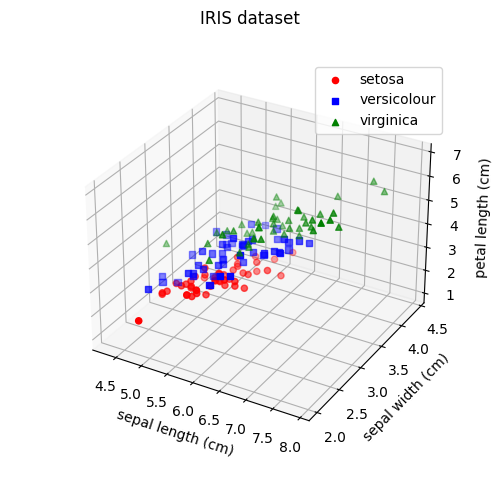
\includegraphics[width=40mm]{iris_3d.png}
        \end{center}
        \caption{解析する元データ(3d)}
        \label{img:iris_3d}
    \end{minipage}
    \begin{minipage}{0.33\hsize}
        \begin{center}
            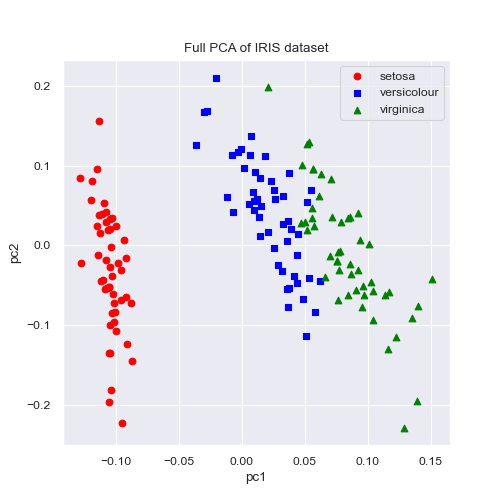
\includegraphics[width=40mm]{iris_full_pca.png}
        \end{center}
        \caption{通常のPCA結果}
        \label{img:iris_full_pca}
    \end{minipage}
    \begin{minipage}{0.33\hsize}
        \begin{center}
            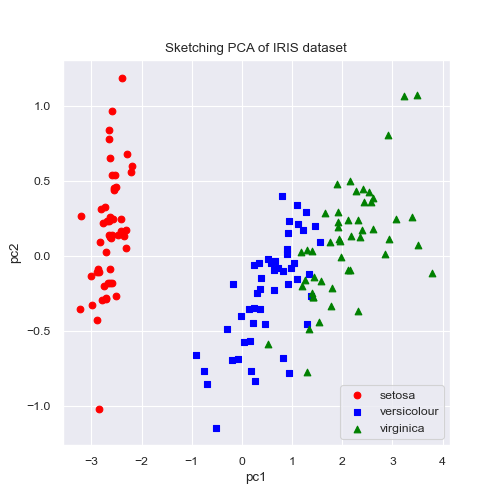
\includegraphics[width=40mm]{iris_sketching_pca.png}
        \end{center}
        \caption{sketchingによるPCA結果}
        \label{img:iris_sketching_pca}
    \end{minipage}
\end{figure}

このコードの計算量はほぼnnzオーダーであるが、先述の通り、他の手法でも特異値分解が高速に出来てしまうので、速度面で圧倒的な優位性があるとは言えないかも知れない。しかし、先程も触れた``streaming''という特性を持ち、並列に実行可能である点で、大規模データに対しては、より優位性を持つと言えるだろう。

このように、本手法は、sketchingと特異値分解の双方にとって、重要な応用例であると言える。

以上で、本課題への解答を終了する。

\newpage

\bibliographystyle{jplain}
\bibliography{applyingForGraduateSchool.bib}

\end{document}
